\newpage
\section{Iteración 0: Decisiones preliminares}
\subsection{Introducción}
En esta iteración vamos plantear la elección que realizamos para todos los componentes que componen el robot, los opciones que contemplamos para la implementación y el motivo de las elecciones.

\subsection{Requerimientos}

En esta iteración abordaremos los siguientes requerimientos funcionales:

\begin{center}
    \begin{tabular} {
        | >{\centering\arraybackslash}m{1cm}
        | >{\centering\arraybackslash}m{13cm} |}
        \hline \rowcolor{test_header_color}
            ID & Descripción \\
        \hline
            RF4 & El robot debe poder realizar trayectorias en línea recta y curvas. \\
        \hline
            RF6 & El robot debe recibir y enviar información mediante comunicaciones inalámbricas. \\
        \hline
            RF8 & Debe poder ubicarse al robot en el plano de forma precisa. \\
        \hline
    \end{tabular}
\end{center}

   Por otra parte, el requerimiento no funcional que abordaremos es:

\begin{center}
    \begin{tabular} {
        | >{\centering\arraybackslash}m{1cm}
        | >{\centering\arraybackslash}m{13cm} |}
        \hline \rowcolor{test_header_color}
            ID & Descripción \\
        \hline
            RNF1 & Debería tener tiempos de respuesta aceptables para el buen funcionamiento del sistema de control. \\
        \hline
    \end{tabular}
\end{center}

\subsection{Desarrollo}

\subsection{Relevamiento del Proyecto Integrador Hermes III}

El robot Hermes III es la última versión de la familia de robots desarrollada dentro del laboratorio de arquitectura de computadoras. Este también incorpora sistemas del modelo anterior y plantea una mejora sobre ellos, en este caso sobre el sistema de control que comanda el robot móvil y la implementación de un sistema operativo robótico (ROS) el cual es un framework para Linux que está diseñado exclusivamente para el desarrollo de robots. \cite{micolini2022hermes}

El uso del sistema operativo ROS abre la posibilidad de usar software dedicado al desarrollo de robots móviles y también a la incorporación de componentes como ser el módulo de cámara Kinect desarrollado por Microsoft para la consola Xbox.

El conjunto ya mencionado da paso a la implementación e innovación más importante del proyecto, la localización y mapeo en simultáneo (SLAM), brindándole al robot la posibilidad de moverse sobre un superficie y crear un mapa de su entorno, provocando que en cada nueva iteración pueda mejorar su desplazamiento y localización en la superficie de movimiento.

El software se ejecuta sobre una placa NVIDIA Jetson TK1, la cual ofrece un gran poder de cómputo que es necesario para sostener y correr de forma efectiva tanto el sistema operativo como el algoritmo de SLAM. La desventaja es su alto precio, lo que aumenta el costo de construcción del robot y por lo tanto disminuye la posibilidad de pensar en un flota de estos equipos.

\subsubsection{Elección de microcontrolador}

Dentro de las características del modelo anterior de la familia Hermes, se destacaba la gran cantidad hardware por el cual estaba compuesto, y por ende, el gran costo para su replicación e implementación.

Para esta nueva edición se decidió reducir la cantidad de componentes que lo integran, en cuanto al procesamiento se refiere, y llevarlo a un modelo que se acerque mas a la Industria 4.0 donde los dispositivos se conectan a Internet y es allí donde mandan reportes y reciben instrucciones. Es por eso que se optó por la utilización del microcontrolador ESP-32 el cual proporciona un API bastante completa y por en ende un gran abanico para que el desarrollador despliegue todo su potencial. \cite{kolban2017kolban}

\begin{figure}[H]
   \centering
   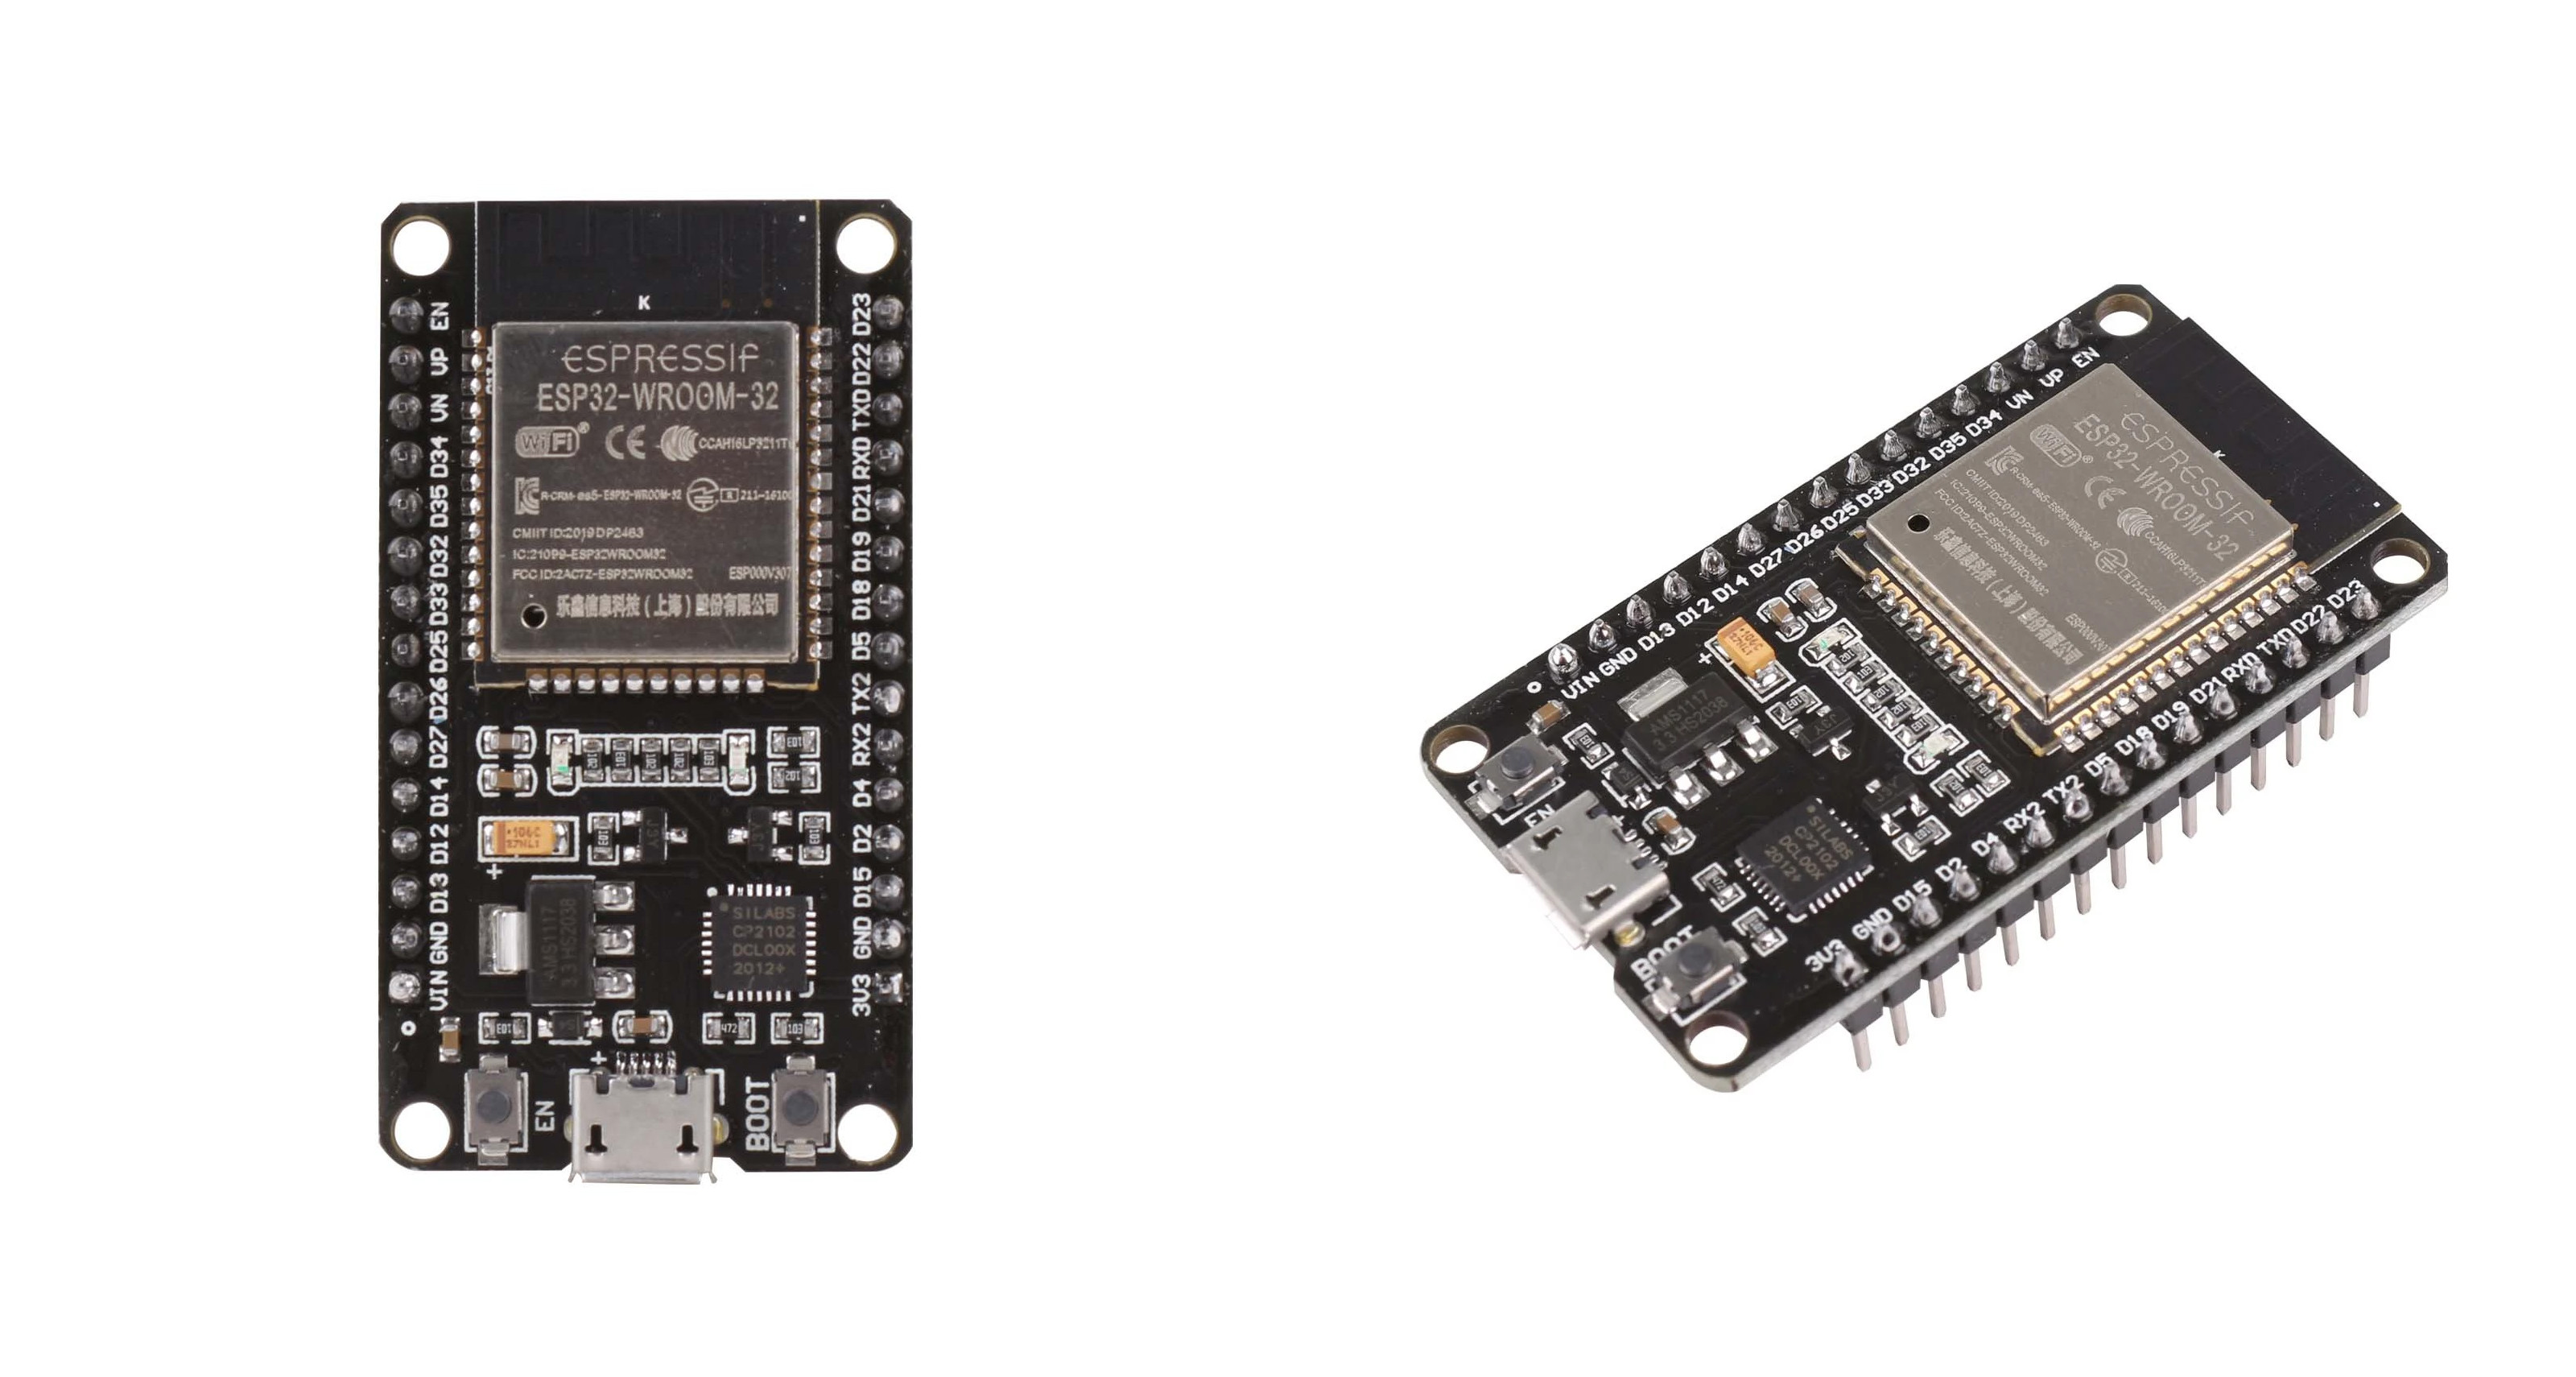
\includegraphics[width=0.7\linewidth]{images/esp32-micro.jpg}
   \caption{Microcontrolador ESP32}
   \label{fig:microcontrolador}
\end{figure}

\subsubsection{Sistema Operativo}

La decisión de utilizar FreeRTOS como sistema operativo para el desarrollo de este proyecto se fundamenta en varias consideraciones claves. Primero, FreeRTOS está integrado de manera nativa en el framework ESP-IDF de Espressif, lo que facilita enormemente el desarrollo y la integración de funcionalidades en tiempo real. Al utilizar la API de Espressif, se aprovechan componentes y servicios que ya están optimizados para trabajar con FreeRTOS, lo que se traduce en una mayor estabilidad y rendimiento en aplicaciones críticas.

FreeRTOS permite una gestión eficiente de tareas, permitiendo la concurrencia y la sincronización de procesos de manera robusta y controlada. Esto es esencial para aplicaciones que requieren una respuesta rápida a eventos externos, como la gestión de sensores, la comunicación inalámbrica y la realización de múltiples operaciones simultáneamente. La modularidad y escalabilidad que ofrece FreeRTOS permite desarrollar soluciones complejas sin incurrir en sobre costos de recursos, lo que es especialmente valioso en sistemas embebidas con limitaciones de hardware. \cite{barry2016mastering}

El uso de FreeRTOS está respaldado por un amplio ecosistema de documentación y soporte, facilitando el desarrollo, la depuración y el mantenimiento de aplicaciones en el microcontrolador ESP32. Esta sinergia entre el hardware y el sistema operativo garantiza una integración fluida y optimizada para las exigencias de aplicaciones modernas en sistemas embebidos y soluciones IoT, lo que se ajusta perfectamente al desarrollo de este proyecto.

\begin{figure}[H]
  \centering
  
\includegraphics[width=0.4\linewidth]{images/freertos.jpg}
  \caption{Sistema operativo usado por los microcontroladores}
  \label{fig:sistema_operativo}
\end{figure}

\subsubsection{Elección de motores}

El sistema de locomoción es el responsable de la traslación del robot. Las configuraciones más comunes son las siguientes: diferencial, sincrónico, triciclo, ackerman y omnidireccional.

Como nosotros tomamos como base la estructura ya definida para el robot Hermes III, adoptamos el sistema mecánico de locomoción omnidireccional, el cual permite mayor libertad de movimiento que los sistemas de ruedas clásicos, Los robots que implementan este sistema pueden moverse en cualquier dirección sobre el plano y en cualquier momento sin la necesidad de hacer movimientos previos para modificar su trayectoria. Requiere ruedas que permitan movimientos en más de una dirección. Este sistema puede ser implementado con tres o cuatro ruedas.

Las ruedas omnidireccionales ruedan en el sentido de avance, pero, también se pueden desplazar lateralmente con gran facilidad como se observa en la siguiente figura:

\begin{figure}[H]
    \centering
    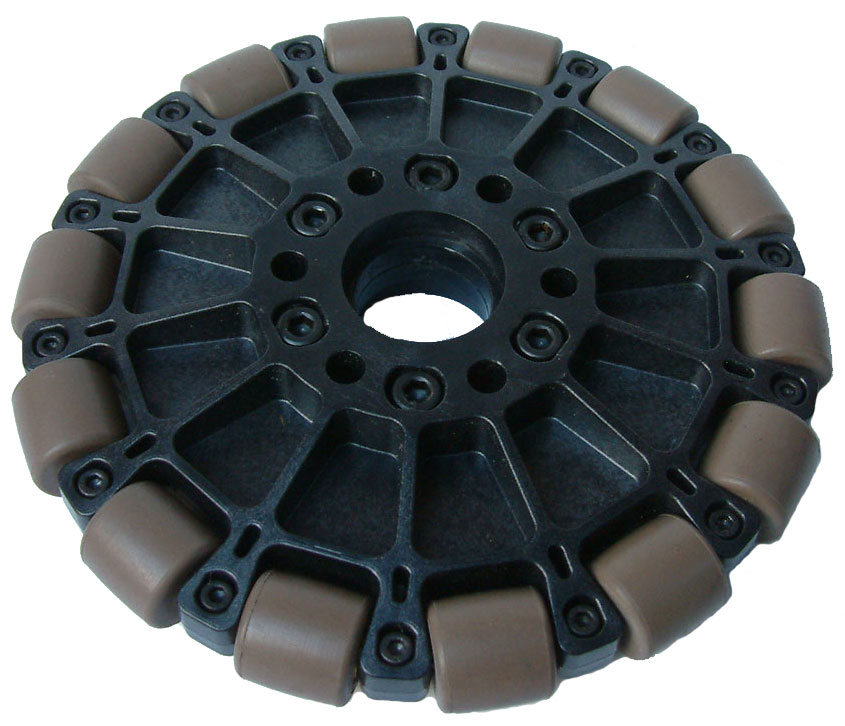
\includegraphics[width=0.25\linewidth]{images/omni-wheel-wikipedia.png}
    \caption{Rueda omnidireccional}
    \label{fig:rueda_omnidireccional}
\end{figure}

Los actuadores tienen por misión generar el movimiento de los elementos del robot según las órdenes dadas por la unidad de control. De manera general, los actuadores utilizados en robótica pueden emplear energía neumática, hidráulica o eléctrica. Las características de control, sencillez y precisión de los accionamientos han hecho que los actuadores eléctricos sean los más usados. Dentro de los actuadores eléctricos pueden distinguirse tres tipos diferentes: \\

\textbf{Motores de corriente continua (DC):}
\begin{itemize}
   \item Controlados por inducción
   \item Controlados por excitación
\end{itemize}

\textbf{Motores de corriente alterna (AC):}
\begin{itemize}
   \item Síncronos
   \item Asíncronos
\end{itemize}

Se opta por motores de corriente continua, como el que se muestra en la figura siguiente, pues el torque generado es proporcional a la diferencia de potencial aplicado a los terminales de alimentación y el sentido de giro depende de la polaridad, facilitando de este manera el control. El modelo de motor elegido se muestra en la imagen debajo, es un motorreductor de $12V\ @\ 100\ RPM$.

\begin{figure}[H]
    \centering
    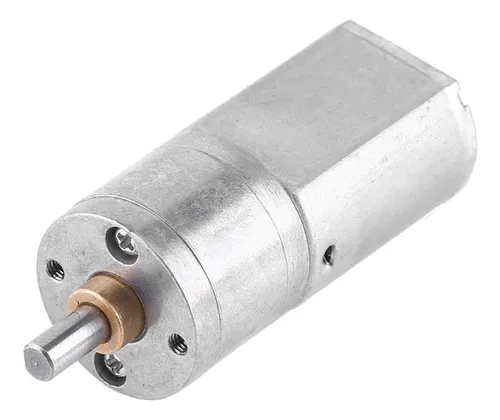
\includegraphics[width=0.35\linewidth]{images/motorreductor.png}
    \caption{Motorreductor}
\end{figure}


Este tipo de motores pequeños y de bajo costo generalmente presentan como inconveniente que no publican sus curvas. Para resolver este inconveniente se realizaron distintos experimentos. Esencialmente se construyó un montaje que consta de una polea con un peso conocido, que no es más que un recipiente con agua como muestra la siguiente figura, la polea se fija al eje del motor para realizar los experimentos.

Se realizaron distintas corridas variando la tensión y corriente, se tomaron mediciones de velocidad y torque. Con estos datos se construyeron las curvas de rpm-torque y corriente-torque, como se muestra la siguiente tabla:

\begin{center} \begin{tabular}{|c|c|c|}
   \hline \rowcolor{test_header_color}
       Tensión & Velocidad & Torque \\
   \hline
       3V & 25 RPM & 0,3 Kg*cm\\
   \hline
       6V & 67 RPM & 1 Kg*cm\\
   \hline
       12V & 96 RPM & 2 Kg*cm\\
   \hline
\end{tabular} \end{center}

Con estos experimentos, también, se midió la respuesta del sistema a un escalón, detallado en la siguiente iteración.

\begin{figure}[H]
    \centering
    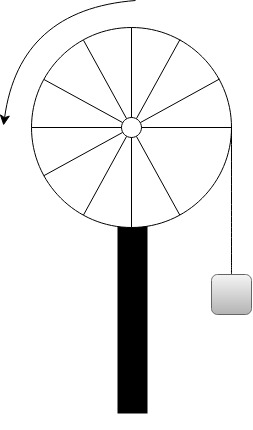
\includegraphics[width=0.25\linewidth]{images/medicion_rpm.jpg}
    \caption{Montaje para medir el torque}
    \label{fig:medicion_torque}
\end{figure}

Para la alimentación de los motores es necesario un circuito integrado especial que permite manipular de manera segura la corriente eléctrica de los motores y a su vez brinde la posibilidad de controlar la polaridad de los bornes donde se conectan los mismos para cambiar su sentido de giro.

Esta solución se ofrece en el mercado en el integrado comúnmente denominado "Driver Dual para Motores L298N", también conocido como "puente H", el cual posee a su vez un regulador de voltaje LM7805 para alimentar la parte lógica del integrado L298N.

El sentido de giro de un motor estará definido por dos pines cuyos valores establecerán la polaridad de los terminales de alimentación del motor respectivamente. Existen dos pares de pines por cada motor.

Para el control de estos integrados vamos a usar cuatro canales PWM del microcontrolador ESP-32, los cuales van a establecer el sentido de giro y fuerza del motor.

\subsubsection{Sensores rotativos} \mbox{} \vspace{10pt} \\
Un sensor es un dispositivo eléctrico y/o mecánico capaz de convertir magnitudes físicas, como la luz, velocidad, aceleración, presión, temperatura, etc. En otra magnitud, normalmente eléctrica, que sea posible manipular y cuantificar.

Para nuestro caso en particular, usamos los sensores para medir la velocidad de los motores. Como el objetivo es construir un sistema de lazo cerrado que controle la velocidad de los motores con el fin de aproximar la trayectoria calculada.

Para medir la velocidad en revoluciones por minuto (RPM), se colocó, en el eje del motor, una rueda con patrón impreso el cual es detectado por un sensor infrarrojo (opto acoplador de ranura). El patrón impreso consta de líneas perforadas, ranuras, en la rueda con el fin de generar interrupciones. Se realizaron 24 ranuras en cada rueda para poder realizar el cálculo de la distancia recorrida.

Para realizar la medición de RPM se experimentó tres métodos diferentes:

\begin{itemize}
   \item Generando una interrupción con el flanco de señal obtenida del sensor infrarrojo. Las RPM se determinan en función de la cantidad de interrupciones contadas en el periodo de una base de tiempo implementada para este fin.
   \item Tomando el tiempo del sistema entre dos interrupciones consecutivas, y luego calcular las RPM.
   \item Midiendo la cantidad de pulsos generada por una base de tiempo externa entre dos interrupciones. Para lo cual se toma la lectura de un contador en la primera interrupción y se toma la lectura nuevamente en la interrupción siguiente. Con la diferencia entre las lecturas se calculan las RPM.
   \item Utilizando el contador de pulso incorporado en el microcontrolador ESP32, y para tener en cuenta las bajas revoluciones acumular los pulsos para luego calcular el promedio y obtener un resultado más preciso.
\end{itemize}

\begin{figure}[H]
  \centering
  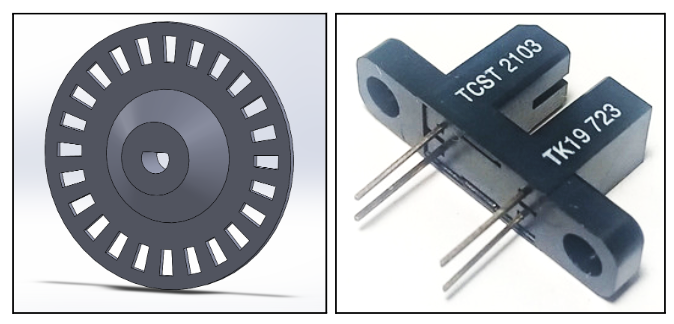
\includegraphics[width=0.7\linewidth]{images/encoder.png}
  \caption{Modelo 3D del encoder rotativo y opto acoplador de ranura}
  \label{fig:encoder}
\end{figure}

Por último se debe destacar que es necesario filtrar el rebote de los flancos de subida y bajada en cada interrupción.

\subsubsection{Elección de lenguaje para interfaz} \mbox{} \vspace{10pt} \\
En cuanto a las elección del lenguaje se refiere, teníamos dos caminos para elegir, ya que nos encontrábamos limitados por el microcontrolador que soporta tanto C como microPython. Habiendo hecho un análisis y una lectura de las distintas APIs que el fabricante nos ofrece, optamos por C ya que es un lenguaje conocido por nosotros. Esto porque durante el transcurso de la carrera nos tocó desarrollar varios trabajos prácticos en este lenguaje, por lo que sentíamos que no necesitabamos adquirir muchos nuevos conocimientos, es un entorno cómodo para trabajar y la documentación es que se encuentra es amplia por lo que los problemas que podían llegar a surgir los íbamos a poder sortear con cierta facilidad.
En el escenario de seguimiento del robot nos encontramos con el desafió de realizar una interfaz amigable, entendible y que pueda desarrollarse de la forma mas rápida posible sin la necesidad de tener una curva de aprendizaje muy grande. Es por ello que optamos por Python para poder cumplir todos los requisitos ya mencionados. Ambos integrantes ya habíamos trabajado con este lenguaje, y ademas, últimamente, se lo encuentra seguido entre los lenguajes mas utilizados por toda la comunidad de la programación, esto por ser un lenguaje sumamente adaptable ante cualquier necesidad y contar con una variedad muy extensa de librerías. Nos pareció una buena elección que nos daba la opción de sortear cualquier obstáculo que surgiera en el camino.

\subsubsection{Comunicación inalámbrica}

Nuestro proyecto al estar pensado para cumplir con los estándares de la Industria 4.0, nos vimos en la necesidad de incorporar la comunicación inalámbrica como medio principal para poder conectar y establecer comunicación entre los distintos componentes que forman parte del proyecto. Así como muestra el diagrama de alto nivel, los componentes se comunican utilizando un router como medio para poder llegar uno hacia otro.

Los microcontroladores elegidos vienen incorporados con los integrados necesarios para hacer uso de esta tecnología y ademas cuentan con la posibilidad de incorporarles una antena, lo que mejora la calidad de la señal y amplia su rango de alcance por lo que los vuelve mas efectivos aun si es que se necesita enviar gran cantidad de información y asegurar que los paquetes van a llegar a destino.

Existe la posibilidad de usar protocolos propios de estos microcontroladores, como ser ESP-NOW, para establecer una comunicación mas segura entre los microcontroladores, pero, optamos por hacer uso del protocolo MQTT que es usado ampliamente en la industria para enviar información de sensores y mensajes cortos. Esto debido a la liviandad y eficiencia de sus mensajes, además, de no atarnos por completo a un protocolo privativo de la marca ESP y poder usar lo que hasta ahora viene siendo un estándar para los dispositivos IoT.

\begin{figure}[H]
   \centering
   
\includegraphics[width=0.7\linewidth]{images/com_inalambrica.jpg}
   \caption{Protocolos usados comúnmente en entornos IoT}
   \label{fig:mqtt}
\end{figure}

\subsection{Testing y pruebas}

Las pruebas que se realizaron para que efectivamente podamos determinar el correcto funcionamiento del Monitor, la gestión de la cola de cortesía y la resolución de conflictos mediante la aplicación de una Política fue con la ayuda de la Red de Petri sumamente conocida como Productor-Consumidor. Esta se tomó cómo referencia ya que permite evaluar los problemas de sincronización, concurrencia y gestión de los recursos, entonces, nos pareció un buen puntapié para validar el funcionamiento con un modelo conocido y sumamente usado. Cabe destacar que realizamos la simulación sobre esta red alrededor de $1M$ de disparos y por supuesto siempre validando el resultado de los $P\ invariantes$ y $T\ invariantes$.

\begin{figure}[H]
   \centering
   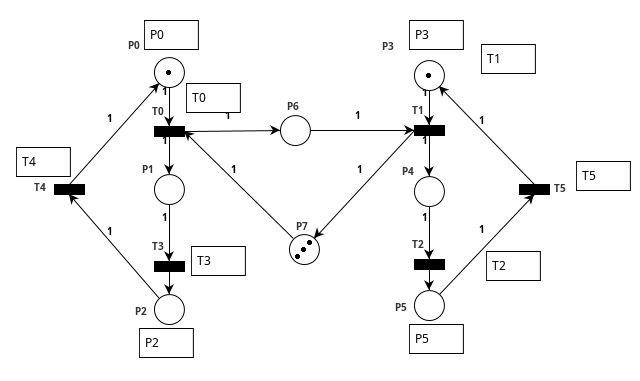
\includegraphics[width=0.9\linewidth]{images/rdp_prod_cons.png}
   \caption{Red de Petri productor-consumidor}
   \label{fig:rdp_prod_cons}
\end{figure}

Se plantearon los siguientes casos:

\begin{testtableformat}
   \hline \rowcolor{test_header_color}
       Test ID             & TC\_04\_00 \\
   \hline
       Tipo de test        & Test unitario \\
   \hline
       Objeto de prueba    & Disparar las transiciones sensibilizadas del Productor \\
   \hline
       Nombre              & Ejecución del productor \\
   \hline
       Descripción         & Realizar el disparo de las transiciones sensibilizadas del productor teniendo como máximo 3 (tres) tokens disponibles para producir\\
   \hline
       Precondición        & PRECOND\_D \\
   \hline
       Pasos del test      & \begin{enumerate}
                             \item Instanciar a la clase monitor con la red productor-consumidor
                             \item Obtener el vector de transiciones sensibilizadas 
                             \item Ejecutar un disparo de la transición sensibilizada 
                             \item Adquirir el marcado saliente y compararlo con un programa de análisis de redes de Petri 
                             \end{enumerate}\\
   \hline
       Resultado esperado  & El marcado en ambos casos debe coincidir \\
   \hline
       Resultado obtenido  & El marcado de la red obtenido por la clase monitor y el programa de análisis de redes de Petri son iguales, por lo tanto, se verifica su adecuado funcionamiento \\
   \hline
       Observaciones       & -\\
   \hline
\end{testtableformat}

\begin{testtableformat}
   \hline \rowcolor{test_header_color}
       Test ID             & TC\_04\_01 \\
   \hline
       Tipo de test        & Test unitario \\
   \hline
       Objeto de prueba    & Disparar las transiciones sensibilizadas del consumidor \\
   \hline
       Nombre              & Ejecución del consumidor \\
   \hline
       Descripción         & Realizar el disparo de las transiciones sensibilizadas del consumidor teniendo como máximo 3 (tres) recursos disponibles generados por el productor\\
   \hline
       Precondición        & PRECOND\_D \\
   \hline
       Pasos del test      & \begin{enumerate} 
                             \item Instanciar a la clase monitor con la red productor-consumidor 
                             \item Obtener el vector de transiciones sensibilizadas 
                             \item Ejecutar un disparo de la transición sensibilizada 
                             \item Adquirir el marcado saliente y compararlo con un programa de analisis de redes de petri 
                             \end{enumerate}\\
   \hline
       Resultado esperado  & El marcado en ambos casos debe coincidir \\
   \hline
       Resultado obtenido  & El marcado de la red obtenido por la clase monitor y el programa de análisis de redes de Petri son iguales, por lo tanto, se verifica su adecuado funcionamiento \\
   \hline
       Observaciones       & -\\
   \hline
\end{testtableformat}

\begin{testtableformat}
   \hline \rowcolor{test_header_color}
       Test ID             & TC\_04\_02 \\
   \hline
       Tipo de test        & Test unitario \\
   \hline
       Objeto de prueba    & Disparar una transición con política de decisión \\
   \hline
       Nombre              & Ejecución de una transición con política definida \\
   \hline
       Descripción         & En en el caso donde tanto el productor cómo el consumidor pueden disparar una transición, la idea es evaluar la política de la transición del consumidor para que tenga prevalencia sobre el productor ante una situación indeterminista \\
   \hline
       Precondición        & PRECOND\_E \\
   \hline
       Pasos del test      & \begin{enumerate} 
                             \item Instanciar a la clase monitor con la red productor-consumidor 
                             \item Generar una situación de equidad donde ambos recursos puedan disparar su transición 
                             \item Obtener el vector de transiciones sensibilizadas 
                             \item Evaluar la política de las transiciones sensibilizada y elegir cual disparar 
                             \item Ejecutar un disparo de la transición elegida 
                             \item Adquirir el marcado saliente y compararlo con un programa de análisis de redes de petri 
                             \end{enumerate}\\
   \hline
       Resultado esperado  & El marcado actual en ambos casos debe coincidir y la transición disparada debe ser la del consumidor \\
   \hline
       Resultado obtenido  & El marcado de la red obtenido por la clase monitor y el programa de análisis de redes de Petri son iguales, por lo tanto, se verifica su adecuado funcionamiento \\
   \hline
       Observaciones       & -\\
   \hline
\end{testtableformat}

\begin{testtableformat}
   \hline \rowcolor{test_header_color}
       Test ID             & TC\_04\_03 \\
   \hline
       Tipo de test        & Test integración \\
   \hline
       Objeto de prueba    & Realizar movimientos con el robot dentro del mapa, el robot sólo va a avanzar cuando la red de Petri haya hecho la solicitud de disparo y haya verificado que el robot no se encuentra bloqueado.\\
   \hline
       Nombre              & Desplazamientos del robot controlado por el Monitor\\
   \hline
       Descripción         & Para que el robot avance de una celda a otra y realice el desplazamiento definido (punto inicial y final) debe ser autorizado y coordinado por el monitor que controla la red de Petri.\\
   \hline
       Precondición        & PRECOND\_E \\
   \hline
       Pasos del test      & \begin{enumerate}
                             \item Indicar los puntos de inicio y final del robot
                             \item Esperar que el Monitor dispare la transición sensibilizada
                             \item El robot recibe la orden de avanzar a la celda libera
                             \item El robot envía una señal de llegada a la celda (plaza)
                             \item Se dispara la siguiente transición sensibilizada
                             \item Este proceso se repite hasta que el robot llegue a su destino
                             \end{enumerate}\\
   \hline
       Resultado esperado  & El robot pueda completar su desplazamiento definido por el usuario\\
   \hline
       Resultado obtenido  & La red de Petri al no bloquearse permite que todas las transiciones sensibilizadas se puedan disparar y por ende que el robot pueda desplazarse por todas las celdas (plazas) involucradas en su recorrido\\
   \hline
       Observaciones       & -\\
   \hline
\end{testtableformat}

\begin{testtableformat}
    \hline \rowcolor{test_header_color}
        Test ID             & TC\_04\_04 \\
    \hline
        Tipo de test        & Test de sistema \\
    \hline
        Objeto de prueba    & Comunicación inalámbrica - PID - Modelo cinemático - Odometría - Seguidor de línea magnética - Modelo del mapa - Calculador de trayectorias - Interfaz de usuario - Red de Petri - Monitor \\
    \hline
        Requerimiento       & RF1 - RF2 - RF3 - RF4 - RF5 - RF6 - RF7 - RF10 \\
    \hline
        Nombre              & Prueba de sistema integrado\\
    \hline
        Descripción         & Comprobar que el robot se puede desplazar por el mapa gestionado por el marcado de la red de Petri\\
    \hline
        Precondición        & PRECOND\_G \\
    \hline
        Pasos del test      & \begin{enumerate}
                              \item Indicar los puntos de inicio y final del robot en el mapa
                              \item Calcular la secuencia de disparos del Monitor
                              \item Esperar que el Monitor dispare la transición sensibilizada
                              \item El robot recibe la orden de avanzar a la celda (plaza) liberada
                              \item El robot envía una señal de llegada a la celda (plaza) destino
                              \item Se dispara la siguiente transición sensibilizada
                              \item Este proceso se repite hasta que el robot llegue a su destino
                              \end{enumerate}\\
    \hline
        Resultado esperado  & El robot pueda completar su desplazamiento definido por el usuario\\
    \hline
        Resultado obtenido  & La red de Petri al no bloquearse permite que todas las transiciones sensibilizadas se puedan disparar y por ende que el robot pueda desplazarse por todas las celdas (plazas) involucradas en su recorrido\\
    \hline
        Observaciones       & Se probó recorridos de 4 de metros por limitaciones de espacio\\
    \hline
 \end{testtableformat}

\subsection{Resultados}
El resultado es satisfactorio debido a que pudimos recolectar gran cantidad de información de todos los componentes y armamos el principio de lo que será el desarrollo de todo el proyecto.

\subsection{Riesgos superados}
\begin{center}
    \begin{tabular} {
        | c| c |}
        \hline
            ID & Riesgo \\
        \hline
            RI-04 & Modificación de los requerimientos del proyecto\\
        \hline
    \end{tabular}
\end{center}

\subsection{Conclusiones}
En base a los información recolectada y leída, vemos que planteamos una base por donde comenzar el proyecto, definiendo los sistemas y componentes que se van a usar para su implementación, por lo tanto nos sentimos cómodos con las decisiones tomadas y vemos con buenos ojos el comienzo del desarrollo.